\documentclass[reprint,english,notitlepage]{revtex4-2}
\usepackage{amsmath}
\usepackage[mathletters]{ucs}
\usepackage[utf8x]{inputenc}
\usepackage[english]{babel}
\usepackage{esint}
\usepackage{physics,amssymb}
\usepackage{graphicx}
\usepackage{xcolor}
\usepackage{hyperref}
\usepackage{listings}
\usepackage{subfigure}
\usepackage[style=science, backend=biber]{biblatex}
\usepackage{booktabs}
\addbibresource{References_Part_4.bib}
\hypersetup{
    colorlinks,
    linkcolor={red!50!black},
    citecolor={blue!50!black},
    urlcolor={blue!80!black}}

\lstset{inputpath=,
	backgroundcolor=\color{white!88!black},
	basicstyle={\ttfamily\scriptsize},
	commentstyle=\color{magenta},
	language=Python,
	morekeywords={True,False},
	tabsize=4,
	stringstyle=\color{green!55!black},
	frame=single,
	keywordstyle=\color{blue},
	showstringspaces=false,
	columns=fullflexible,
	keepspaces=true}


\begin{document}



\title{Onboard Orientation Software}
\author{Oskar Idland \& Jannik Eschler}
\date{\today}
\affiliation{Institute of Theoretical Astrophysics, University of Oslo}

\begin{abstract}
    This is an abstract \colorbox{red}{Complete this summary at the end of the paper}
\end{abstract}
\maketitle

\section{Introduction} \label{sec:introduction}
As there is no up or down in space we will have to create our own way of navigating the cosmos.
For this purpose, software capable of orientation in space needs to be created.
Without it, we wouldn't be able to steer our spacecraft and reach our destination.
To orient ourselves, three things will be required.\\
To know where our spacecraft is located in the solar system, we need to know our position.
The position can be found using a process called trilateration.\\
Trilateration is the process by which one determines the position of a body using measured distances to known positions.~\parencite[][]{Relevant_theory}\\
This means we can use measure distances from the spacecraft to object for which we know the position and calculate our own position from there.
These measurements will be done by our onboard radar array.\\
The software for the array includes an index of all known objects in our solar system and can therefore include the radius of the object in it's calculations.
The measured distance will therefore always be from the spacecraft to the center of the object.\\
As most objects in space - including the spacecraft itself - are moving, we need to specify the point in time when the measurements were taken.
Otherwise, we could not know the exact location of the object we are measuring the distance to.\\
Furthermore, we need to know in which direction we are moving.
This consists of two parts.
\colorbox{red}{We need to know which way the spacecraft is pointing.} \colorbox{red}{OSKAR}\\
We also need to know the velocity of the spacecraft relative to the star in our solar system.
To find the velocity relative to a star, we can use a phenomenon called Doppler shift.
Electromagnetic radiation consist of waves which have an amplitude and a frequency.
The amplitude determines the intensity of the light, whereas the frequency determines the energy of the wave, or in other words the colour.
If two objects move at high velocities relative to each other and one receives light sent out by the other, the electromagnetic wave appears to be compressed if the objects are moving towards each other and stretched out if they are moving away from each other.
Therefore, the frequency will appear to be higher or lower respectively.
Additionally, relativistic effects distort the wave further due to the relatively high speeds.\\
However, we cannot apply this directly to find our velocity relative to the star in our solar system as this only determines the radial velocity relative to the star and the spacecraft also has a tangential velocity to relative to the star.
We will therefore use reference stars which are outside our solar system.\\
The Doppler shift and therefore the velocity of the reference relative to the star in our solar system is known.
We can then measure the Doppler shift of the reference stars from our spacecraft and determine the velocity of the stars relative to the spacecraft.
Here, we assume the lines from the spacecraft to the reference stars and the lines from the star in our solar system to the reference stars to be parallel due to the reference stars being very far away.\\
These velocities can then be used to find the velocity of the spacecraft relative to the star in our solar system.
Since we are only able to find the radial velocity to the reference star, we will need at least two stars to be able to determine our velocity in two dimensions.\\
As stars mainly consist of hydrogen, most electromagnetic radiation sent out from stars will be from hydrogen atoms sending out radiation.
This spike in the amount of radiation at a specific wavelength is called the $H_{\alpha}$ Spectral Line, which has a wavelength of 656.3 nanometers.\\
To be able to do all calculations, a cartesian coordinate system will be used with the star in our solar system being in the origin and the x-axis pointing at the position of planet 0 at $T = 0$.

\section{Theory} \label{sec:theory}
For theory, see section Relevant Mathematics in the project description~\parencite[][]{Relevant_theory}


\section{Method} \label{sec:method}
\subsection{Creating a picture}\label{subsec:creating-a-picture}
A satellite is orbiting our home planet and has taken a $ 360 ^{o} \times 360 ^{o} $ picture of the entire sky where all positions are described using spherical coordinates. As the stars and galaxies as very far away we are going to assume the pictures looks the same from the perspective of our shuttle. Using this picture we can create a stereographic projection as a means to convert from spherical coordinates to planar coordinates. Comparing the picture taken from a camera at on the shuttle we can find our orientation.
\begin{figure}[h!]
  \centering
  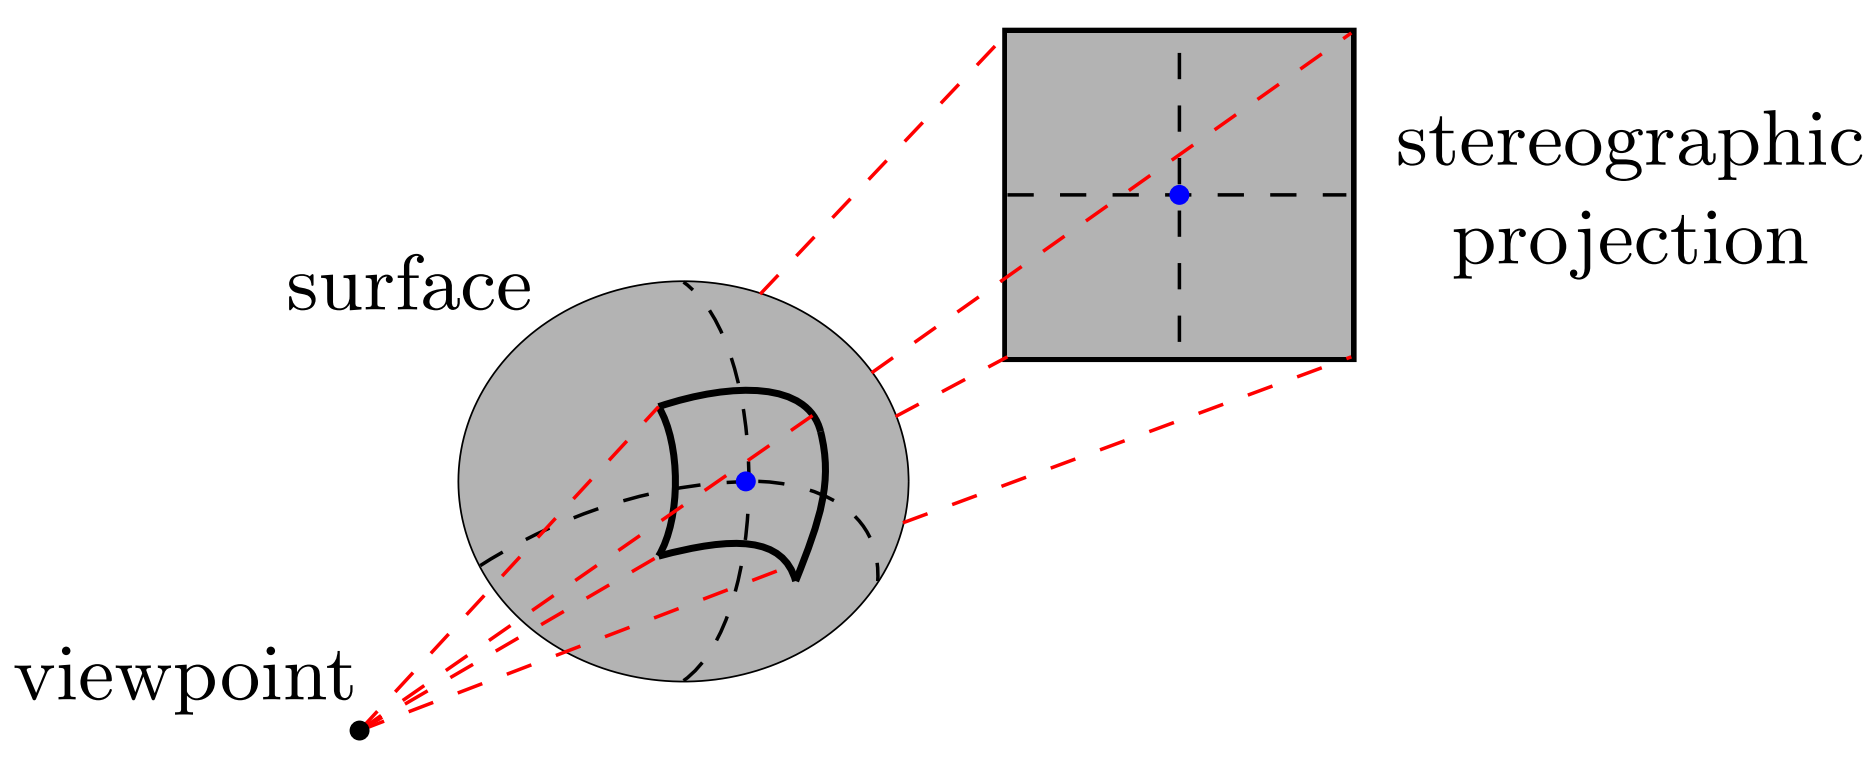
\includegraphics[scale = .2]{Figures/Stereographic_projection}
  \caption{Illustration of stereographic projection}
  \label{fig: Stereographic Projection}
\end{figure}\\
To relate the spherical coordinates $ \theta, \phi $ to the planar coordinates $ X, Y $ we use the following equations \colorbox{red}{Husk å ta med utledning} :
\begin{equation} \label{Spherical to X}
	X = κ  \sin θ \sin (ϕ - ϕ _0)
\end{equation}
\begin{equation}\label{Spherical to Y}
	Y = κ (\sin θ _0 \cos  θ - \cos θ _0 \sin θ \cos (ϕ - ϕ _0))  
\end{equation}

When the camera onboard takes a pictures it will be limited by its field of view (FOV).
The FOV will be described as the maximum angular width $ \alpha $ of the photo.
We use the following equations to define it.
\begin{equation} \label{eq: max angular width}
	α _{\theta} = θ _{max} - \theta _{min}, \quad α _{\phi} = ϕ _{max} - ϕ _{min}
\end{equation}

This creates ranges of coordinates for $\theta$ and $\phi$:
\begin{equation}\label{eq: limitations phi and theta}
  - \frac{\alpha _{\theta}}{2} \le θ - θ _{0} \le \frac{\alpha _{\theta }}{2}, \quad - \frac{\alpha _{\theta}}{2} \le ϕ  - ϕ _{0} \le \frac{\alpha _{\theta }}{2}
\end{equation}

This, in turn, also creates limitations on the coordinates $ (X,Y) $ of the stereographic projection: 
\begin{subequations} \label{eq: limitations X and Y lim}
	\begin{equation}
		X _{max / min} = ± \frac{2 \sin (α _{\phi} / 2)}{1 + \cos (\alpha _{\phi})}
	  \end{equation}
	  
	  
	\begin{equation}
		Y _{max / min} ± \frac{2 \sin (\alpha _{\theta}  / 2)}{1 + \cos (α _{\theta}/2)}
	\end{equation}
	
\end{subequations}




\colorbox{red}{Explain how we made the pixel grid}

\colorbox{red}{Explain how we are gonna generate the picture}





\subsection{Determining the velocity}\label{subsec:determining-the-velocity}
As explained in section~\ref{sec:introduction}, the velocity relative to the star will be determining using an effect called the Doppler shift.
When tasked to do so, the onboard equipment of the spacecraft can now determine the Doppler shift $\Delta \lambda$ of the $H_{\alpha}$ Spectral line.\\
It must be noted that all these measurements will be done at the time $T_M$.\\
The angles from the x-axis at which the reference stars $Star_{R1}$ and $Star_{R2}$ lie are known as $\phi_1 = \colorbox{red}{XXXXXX}$ and $\phi_2 = \colorbox{red}{XXXXXX}$.
These have been obtained beforehand by our astronomers.
Now the velocities $v_{phi1}$ and $v_{phi2}$ in the direction of these angles can be determined by measuring the Doppler shift $\Delta \lambda$ and using the relationship between the Doppler shift and the velocity~\eqref{Dopplershift}
\begin{align}
    \Delta \lambda &= \gamma \left(1 + \frac{v_{rad}}{c}\right) - 1 \label{Dopplershift1}\\
	\Delta \lambda &= \sqrt{\frac{1+\frac{v_{rad}}{c}}{1-\frac{v_{rad}}{c}}} \label{Dopplershift2}
\end{align}
With $\gamma$ being the Lorentz factor, $c$ being the speed of light and $v_{rad}$ being the velocity of the two objects relative to each other.
When rearranging formula~\eqref{Dopplershift2} we obtain a formula for the velocity given a value for the Doppler shift~\eqref{Dopplershift3}.
\begin{align}
    v_{rad} = \frac{-2c}{\left(1+\Delta\lambda \right)^2 +1} + c \label{Dopplershift3}
\end{align}
Given the velocity in the direction of the two stars, we will need to change our coordinate system to calculate the velocity of the spacecraft.
The new unit vectors of our coordinate system will be given by
\begin{align}\label{Coord_chg1}
\begin{pmatrix}
    \hat{u}_1 \\
	\hat{u}_2
\end{pmatrix} =
\begin{pmatrix}
    \cos \phi_1 & \sin \phi_1\\
	\cos \phi_2 & \sin \phi_2
\end{pmatrix}
\end{align}
Now, we are able to determine to calculate the velocity of the spacecraft, and the velocity of the star in our solar system relative to the two reference stars in our new coordinate system.\\
To find the velocity of the spacecraft relative to the star in our solar system, we can simply subtract the velocity of the star in our system from the velocity of the spacecraft.
\begin{align*}
    v_u = v_{SC}-v_{Star}
\end{align*}
However, our orientation system works in cartesian coordinates, so will have to change our coordinate system back to the initial coordinate system.
To change back to the initial system, we invert the operations used in~\eqref{Coord_chg1} and use them on the velocity vector
$v_u = \begin{pmatrix}
    v_{u1}\\ v_{u2}
\end{pmatrix}$.

\begin{align*}
    \begin{pmatrix}
        v_x\\
		v_y
    \end{pmatrix}
	 = \frac{1}{\sin\left(\phi_1 - \phi_2 \right)}
	\begin{pmatrix}
	    \sin\phi_2 & -\sin\phi_1\\
		-\cos\phi_2 & \cos\phi_1
	\end{pmatrix}
	\begin{pmatrix}
		v_{u1}\\ v_{u2}
	\end{pmatrix}
\end{align*}


\subsection{The position of the Spacecraft}\label{subsec:the-position-of-the-spacecraft}




\section{Results} \label{sec:results}



\section{Discussion} \label{sec:discussion}



\section{Conclusion} \label{sec:conclusion}



\section{Appendix: Mathematical Derivations}


\newpage
\newpage
\printbibliography


\end{document}